\subsubsection{Pushbutton Key Parallel Port}

The parallel port connected to the {\it KEY}$_{3-0}$ 
pushbutton switches on the \DEBoard~board comprises three 4-bit
registers, as shown in Figure \ref{fig:pushbutton_port}. These registers have 
the base address {\sf 0xFF200050} and can be accessed using word operations. 
The read-only {\it Data} register provides the values of the switches {\it KEY}$_{3-0}$. 
The other two registers shown in Figure \ref{fig:pushbutton_port}, at addresses
{\sf 0xFF200058} and {\sf 0xFF20005C}, are discussed in Section \ref{sec:exceptions}.
~\\
\begin{figure}[h!]
   \begin{center}
       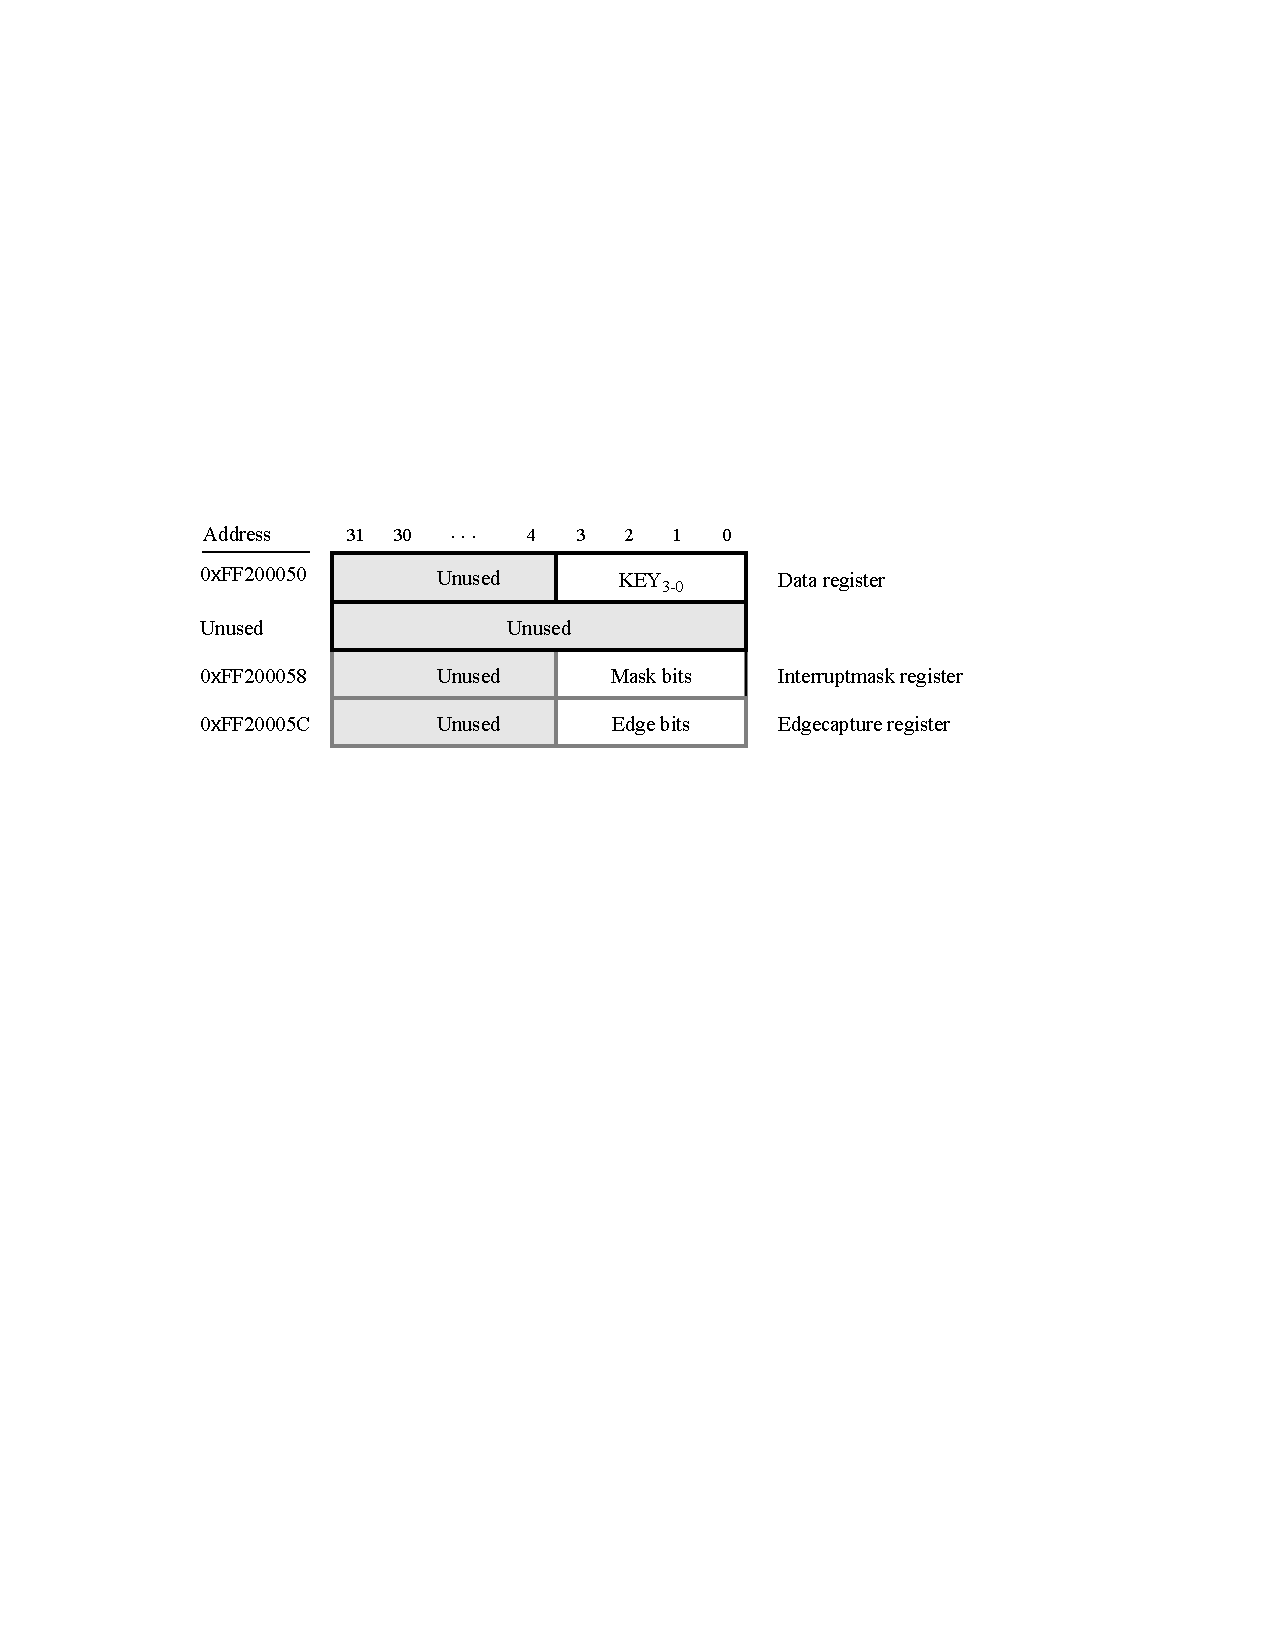
\includegraphics{../../../common/figs/FPGA_PP_Keys_4.pdf}
   \end{center}
   \caption{Registers used in the pushbutton parallel port.}
	\label{fig:pushbutton_port}
\end{figure}


